%-----------------------------------LICENSE------------------------------------%
%   This file is part of tikz_figures.                                         %
%                                                                              %
%   tikz_figures is free software: you can redistribute it and/or              %
%   modify it it under the terms of the GNU General Public License as          %
%   published by the Free Software Foundation, either version 3 of the         %
%   License, or (at your option) any later version.                            %
%                                                                              %
%   tikz_figures is distributed in the hope that it will be useful,            %
%   but WITHOUT ANY WARRANTY; without even the implied warranty of             %
%   MERCHANTABILITY or FITNESS FOR A PARTICULAR PURPOSE.  See the              %
%   GNU General Public License for more details.                               %
%                                                                              %
%   You should have received a copy of the GNU General Public License along    %
%   with tikz_figures.  If not, see <https://www.gnu.org/licenses/>.           %
%------------------------------------------------------------------------------%

% Use the standalone class for displaying the tikz image on a small PDF.
\documentclass[crop, tikz]{standalone}

% Import the tikz package to use for the drawing.
\usepackage{tikz}

% Tikz packages used.
\usetikzlibrary{arrows.meta}

% Begin the document.
\begin{document}

    % Draw the figure.
    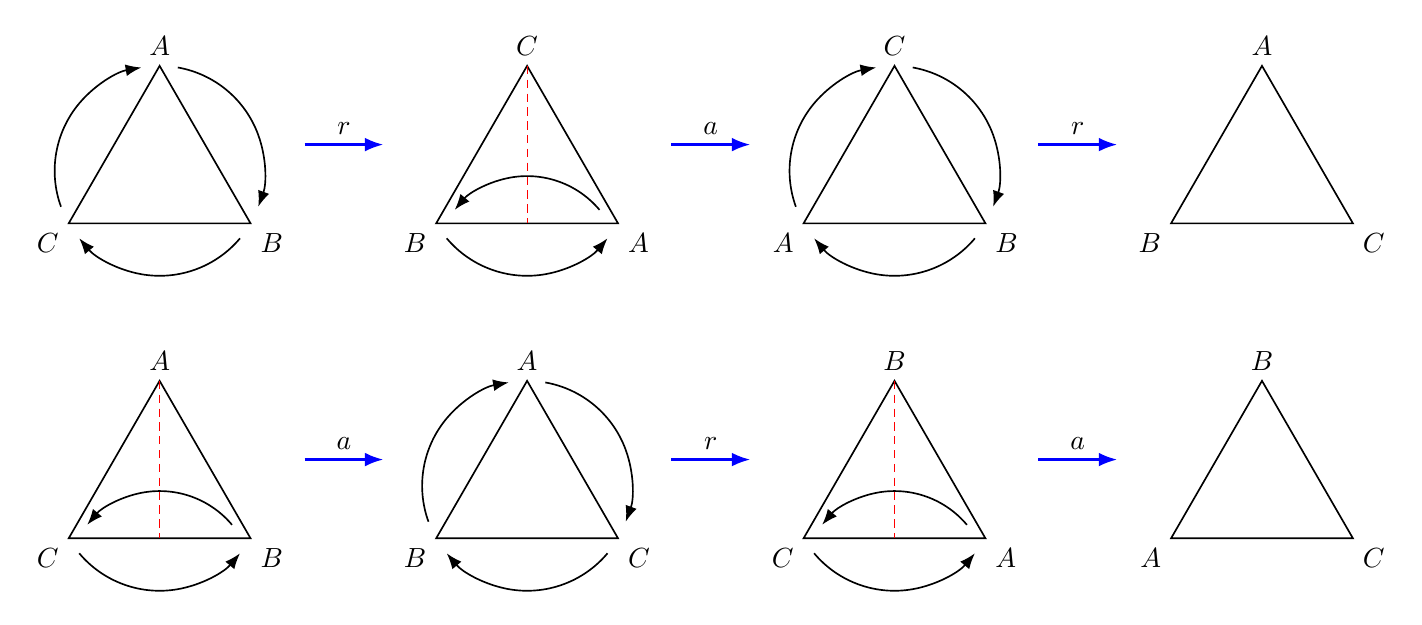
\begin{tikzpicture}[%
        > = Latex,
        p_arc/.style args = {#1:#2:#3}{
            insert path = {+ (#1:#3) arc (#1:#2:#3)},
            ->
        },
        semithick
    ]

        % Command for creating the points on the triangle and drawing it.
        \newcommand*{\defcoords}{%
            \coordinate (O) at (0.0, -0.333333);
            \coordinate (A) at (0.0, 1.0);
            \coordinate (B) at (1.1547, -1.0);
            \coordinate (C) at (-1.1547, -1.0);
            \draw (A) to (B) to (C) to cycle;
        }

        \begin{scope}[xshift = -7.0cm]
            \defcoords;
            \draw (O) [p_arc = 80:-20:1.333];
            \draw (O) [p_arc = -40:-140:1.333];
            \draw (O) [p_arc = 200:100:1.333];
            \node at (A) [above] {$A$};
            \node at (B) [below right] {$B$};
            \node at (C) [below left] {$C$};
        \end{scope}

        \begin{scope}[xshift = -2.333cm]
            \defcoords;
            \draw (O) [p_arc = -140:-40:1.333];
            \draw (0.0, -1.6) [p_arc = 40:140:1.2];
            \draw[densely dashed, thin, red] (0.0, 1.0) to (0.0, -1.0);
            \node at (A) [above] {$C$};
            \node at (B) [below right] {$A$};
            \node at (C) [below left] {$B$};
        \end{scope}

        \begin{scope}[xshift = 2.333cm]
            \defcoords;
            \draw (O) [p_arc = 80:-20:1.333];
            \draw (O) [p_arc = -40:-140:1.333];
            \draw (O) [p_arc = 200:100:1.333];
            \node at (A) [above] {$C$};
            \node at (B) [below right] {$B$};
            \node at (C) [below left] {$A$};
        \end{scope}

        \begin{scope}[xshift = 7.0cm]
            \defcoords;
            \node at (A) [above] {$A$};
            \node at (B) [below right] {$C$};
            \node at (C) [below left] {$B$};
        \end{scope}

        \begin{scope}[draw = blue, ->, thick]
            \draw (-5.16, 00) to node[above] {$r$} (-4.16, 0.0);
            \draw (-0.50, 0.0) to node[above] {$a$} (0.50, 0.0);
            \draw (4.16, 0.0) to node[above] {$r$} (5.16, 0.0);
        \end{scope}

        \begin{scope}[yshift = -4cm]
            \begin{scope}[xshift = -7.0cm]
                \defcoords;
                \draw (O) [p_arc = -140:-40:1.333];
                \draw (0.0, -1.6) [p_arc = 40:140:1.2];
                \draw[densely dashed, thin, red] (0.0, 1.0) to (0.0, -1.0);
                \node at (A) [above] {$A$};
                \node at (B) [below right] {$B$};
                \node at (C) [below left] {$C$};
            \end{scope}
        
            \begin{scope}[xshift = -2.333cm]
                \defcoords;
                \draw (O) [p_arc = 80:-20:1.333];
                \draw (O) [p_arc = -40:-140:1.333];
                \draw (O) [p_arc = 200:100:1.333];
                \node at (A) [above] {$A$};
                \node at (B) [below right] {$C$};
                \node at (C) [below left] {$B$};
            \end{scope}
        
            \begin{scope}[xshift = 2.333cm]
                \defcoords;
                \draw (O) [p_arc = -140:-40:1.333];
                \draw (0.0, -1.6) [p_arc = 40:140:1.2];
                \draw[densely dashed, thin, red] (0.0, 1.0) to (0.0, -1.0);
                \node at (A) [above] {$B$};
                \node at (B) [below right] {$A$};
                \node at (C) [below left] {$C$};
            \end{scope}

            \begin{scope}[xshift = 7.0cm]
                \defcoords;
                \node at (A) [above] {$B$};
                \node at (B) [below right] {$C$};
                \node at (C) [below left] {$A$};
            \end{scope}

            \begin{scope}[draw = blue, ->, thick]
                \draw (-5.16, 0.0) to node[above] {$a$} (-4.16, 0.0);
                \draw (-0.50, 0.0) to node[above] {$r$} (0.50, 0.0);
                \draw (4.16, 0.0) to node[above] {$a$} (5.16, 0.0);
            \end{scope}
        \end{scope}
        \let\defcoords\undefined
    \end{tikzpicture}
\end{document}
